\section{親指基本ポジション}
この章では第VIIポジションよりも高い音を押さえるための「親指基本ポジション」
を紹介します。演奏会で乗る曲の最高音が第7ポジションまでで弾ける場合に
は、この章よりも演奏会の曲の練習を優先して下さい。

\subsection{親指基本ポジションの位置}
ネックの裏から指板の横に出てきた左手の親指が、今度は指板の表にまで出て
きて弦を押さえます。第VIポジションの3の指にあたる位置に親指を置きます。
本書では親指の運指記号として\cite[pp. 5]{streicher2}にならって以下の2つを使用
します。\\

\begin{music}
\nostartrule
\parindent 0pt
\setclef1{\bass}  
\startextract
\NOTEs\zchar{21}{親指でフラジオレット}\enotes
\NOTEs\flag{17}{18}\wh{g}\enotes
\NOTEs\enotes
\doublebar
\NOTEs\zchar{21}{親指で強く押さえる}\enotes
\NOTEs\press{16}{18}\wh{g}\enotes
\notes\enotes
\setdoublebar
\endextract
\end{music}

親指ポジションの指の間隔には主に次の4つの形があります。音符の都合に合わせて使い分けます。

\begin{center}
\begin{tabular}{|l||c|c|c|c|}
\hline
                  & 親指と1の間隔 & 1と2 & 2と3 & 親指と3 \\                
\hline
\hline
クローズ(短三度)形 & 半音    & 半音  & 半音 & 短三度 \\
\hline
長三度形           & 全音    & 半音  & 半音 & 長三度  \\
\hline
完全四度形         & 全音    & 全音  & 半音 & 完全四度 \\
\hline
\end{tabular}
\end{center}

\subsection{クローズ(短三度)形}
クローズ形では全ての指の間隔が半音です。\\
\begin{flushleft}
\begin{minipage}{300pt}
\begin{music}
\nostartrule
\parindent 0pt
\setclef1{\bass}  
\startpiece
\notes\enotes
\Notes\zchar{20}{G線}\flag{16}{17}\wh{g}\zchar{16}{\bf 1}\wh{^g}\zchar{17}{\bf 2}\wh{'a}\zchar{17}{\bf 3}\wh{^a}\enotes
\doublebar
\Notes\flag{16}{17}\wh{g}\zchar{17}{\bf 1}\wh{'_a}\zchar{17}{\bf 2}\wh{=a}\zchar{18}{\bf 3}\wh{_b}\enotes
\doublebar
\Notes\zchar{20}{D線}\flag{13}{14}\wh{d}\zchar{13}{\bf 1}\wh{^d}\zchar{14}{\bf 2}\wh{e}\zchar{15}{\bf 3}\wh{f}\enotes
\doublebar
\Notes\flag{13}{14}\wh{d}\zchar{14}{\bf 1}\wh{_e}\zchar{14}{\bf 2}\wh{=e}\zchar{15}{\bf 3}\wh{f}\enotes
\setdoublebar
\endpiece
\startpiece
\notes\enotes
\Notes\zchar{14}{A線}\flag{10}{11}\wh{a}\zchar{10}{\bf 1}\wh{^a}\zchar{11}{\bf 2}\wh{b}\zchar{12}{\bf 3}\wh{c}\enotes
\doublebar
\Notes\flag{10}{11}\wh{a}\zchar{11}{\bf 1}\wh{_b}\zchar{11}{\bf 2}\wh{=b}\zchar{12}{\bf 3}\wh{c}\enotes
\doublebar
\Notes\zchar{14}{E線}\flag{9}{10}\wh{'E}\zchar{9}{\bf 1}\wh{F}\zchar{9}{\bf 2}\wh{^F}\zchar{10}{\bf 3}\wh{G}\enotes
\doublebar
\Notes\flag{9}{10}\wh{'E}\zchar{9}{\bf 1}\wh{F}\zchar{10}{\bf 2}\wh{_G}\zchar{10}{\bf 3}\wh{=G}\enotes
\setdoublebar
\endpiece
\end{music}
\end{minipage}
\hfill
\begin{minipage}{130pt}
\addtocounter{figure}{1}
\begin{center}
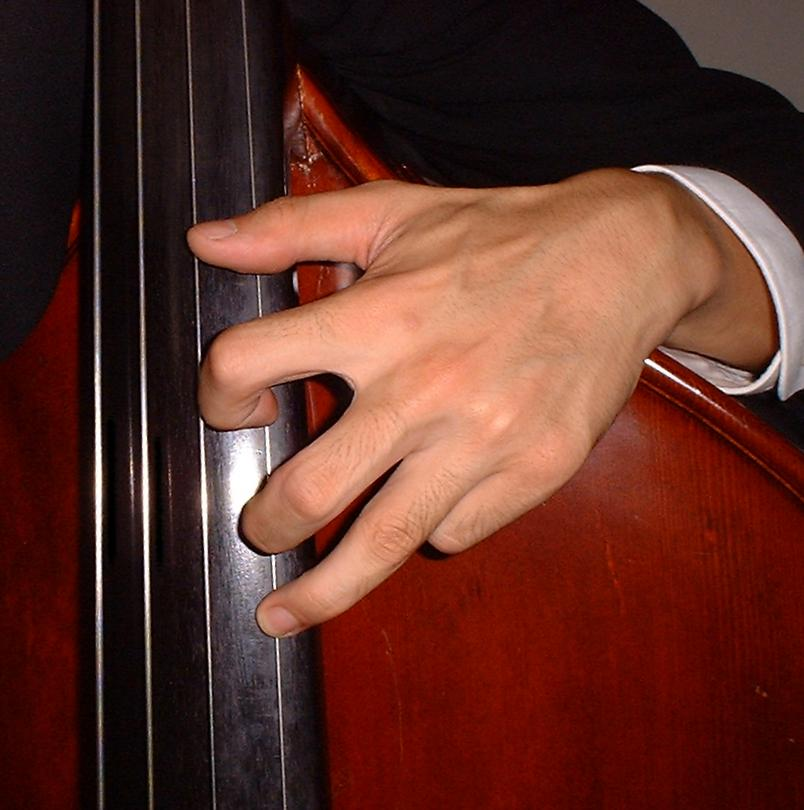
\includegraphics[width=4.5cm]{../Vol1/Pics/Thumb/close.epsi}\\
{\small 図\thefigure : クローズ形は全て半音間隔\\}
\end{center}
\end{minipage}
\end{flushleft}

\subsection{音階練習}

\begin{music}
\nostartrule
\parindent 0pt
\setclef1{\bass}  
\generalsignature{-2}    
\startpiece
\notes\zchar{14}{変ロ長調(B-dur)音階}\enotes
\Notes\zchar{8}{\bf 1}\qu{'B}\enotes
\notes\ibu{0}{'C}{3}\islurd{0}{C}\qb{0}{C}\tbu{0}\tslur{0}{D}\qb{0}{D}\enotes
\notes\ibl{0}{'E}{3}\qb{0}{E}\qb{0}{F}\qb{0}{G}\tbl{0}\qb{0}{!a}\enotes
\bar
\Notes\ql{b}\enotes
\notes\ibl{0}{c}{3}\isluru{0}{c}\zchar{12}{\bf 1}\qb{0}{c}\tbl{0}\tslur{0}{d}\qb{0}{d}\enotes
\notes\ibl{0}{e}{3}\zchar{14}{\bf 1}\qb{0}{e}\qb{0}{f}\flag{16}{17}\qb{0}{g}\tbl{0}\zchar{17}{\bf 2}\qb{0}{'a}\enotes
\bar
\Notes\zchar{18}{\bf 3}\ql{'b}\enotes
\notes\ibl{0}{'a}{-2}\isluru{0}{a}\qb{0}{a}\tbl{0}\tslur{0}{!g}\qb{0}{g}\enotes
\notes\ibl{0}{f}{-3}\zchar{15}{\bf 4}\qb{0}{f}\qb{0}{e}\zchar{13}{\bf 4}\qb{0}{d}\tbl{0}\qb{0}{c}\enotes
\bar
\notes\ibl{0}{b}{-3}\zchar{11}{\bf 4}\qb{0}{b}\qb{0}{a}\qb{0}{'G}\tbl{0}\qb{0}{F}\enotes
\notes\ibu{0}{'E}{-3}\qb{0}{E}\qb{0}{D}\qb{0}{C}\tbu{0}\qb{0}{B}\enotes
\endpiece

\generalsignature{-5}    
\startpiece
\notes\zchar{14}{変ロ短調(b-moll)音階}\enotes
\Notes\zchar{8}{\bf 1}\qu{'B}\enotes
\notes\ibu{0}{'C}{3}\islurd{0}{C}\zchar{8}{\bf 2}\qb{0}{C}\tbu{0}\tslur{0}{D}\qb{0}{D}\enotes
\notes\ibl{0}{'E}{3}\zchar{8}{\bf 1}\qb{0}{E}\qb{0}{F}\qb{0}{=G}\tbl{0}\qb{0}{=!a}\enotes
\bar
\Notes\ql{b}\enotes
\notes\ibl{0}{c}{3}\isluru{0}{c}\zchar{12}{\bf 2}\qb{0}{c}\tbl{0}\tslur{0}{d}\qb{0}{d}\enotes
\notes\ibl{0}{e}{3}\zchar{14}{\bf 1}\qb{0}{e}\qb{0}{f}\flag{16}{17}\qb{0}{=g}\tbl{0}\zchar{17}{\bf 2}\qb{0}{'=a}\enotes
\bar
\Notes\zchar{18}{\bf 3}\ql{'b}\enotes
\notes\ibl{0}{'a}{-2}\isluru{0}{a}\zchar{18}{\bf 1}\qb{0}{_a}\tbl{0}\tslur{0}{!g}\zchar{18}{\bf 4}\qb{0}{_g}\enotes
\notes\ibl{0}{f}{-3}\qb{0}{f}\zchar{14}{\bf 4}\qb{0}{e}\qb{0}{d}\tbl{0}\zchar{12}{\bf 4}\qb{0}{c}\enotes
\bar
\notes\ibl{0}{b}{-3}\qb{0}{b}\zchar{10}{\bf 4}\qb{0}{_a}\qb{0}{'_G}\tbl{0}\zchar{9}{\bf 4}\qb{0}{F}\enotes
\notes\ibu{0}{'E}{-3}\qb{0}{E}\zchar{12}{\bf 4}\qb{0}{D}\qb{0}{C}\tbu{0}\zchar{11}{\bf 1}\qb{0}{B}\enotes
\endpiece
\end{music}

\subsection{親指基本ポジションのクローズ形で弾ける名曲}
\subsubsection*{マーラー: 交響曲第1番 ニ長調 より 第3楽章冒頭}
\begin{music}
\nostartrule
\setclef1{\bass}
\generalsignature{-1}    
\generalmeter{\meterfrac44}
\parindent 0pt
\startbarno=3
\def\writebarno{\tenrm\the\barno\barnoadd}
\def\raisebarno{2\internote}
\def\shiftbarno{0.1\Interligne}
\systemnumbers
\startpiece\bigaccid
\notes\zchar{24}{\bf Feierlich und gemessen, ohne zu schleppen.}\zchar{-5}{\p \ mit D\"{a}mpfer}\enotes
\Notes\isluru{0}{d}\zchar{16}{\downbow}\flag{13}{14}\ql{d}\zchar{16}{\bf 2}\ql{e}\enotes
\notes\ibl{0}{d}{-1}\zchar{19}{\upbow}\zchar{16}{\bf 3}\qb{0}{f}\tbl{0}\qb{0}{e}\enotes
\Notes\tslur{0}{d}\ql{d}\enotes
\notes\cbreath\enotes
\bar
\Notes\isluru{0}{d}\zchar{14}{\downbow}\ql{de}\enotes
\notes\ibl{0}{d}{-1}\zchar{16}{\upbow}\qb{0}{f}\tbl{0}\qb{0}{e}\enotes
\Notes\tslur{0}{d}\ql{d}\enotes
\notes\cbreath\enotes
\bar
\Notes\isluru{0}{f}\zchar{18}{\downbow}\zchar{16}{\bf 3}\ql{f}\flag{20}{21}\ql{g}\tslur{0}{'a}\zchar{21}{\upbow}\zchar{18}{\bf 2}\hl{a}\enotes
\notes\cbreath\enotes
\bar
\Notes\isluru{0}{f}\zchar{16}{\downbow}\ql{fg}\tslur{0}{'a}\zchar{17}{\upbow}\hl{a}\enotes
\notes\cbreath\enotes
\bar
\notes\ibl{0}{e}{-2}\isluru{0}{'a}\zchar{20}{\downbow}\zchar{18}{\bf 2}\qbp{0}{a}\tbbl{0}\zchar{20}{\bf 3}\qb{0}{b}\qb{0}{a}\tbl{0}\flag{20}{21}\qb{0}{!g}\ibl{0}{d}{-2}\zchar{22}{\upbow}\zchar{19}{\bf 3}\qb{0}{f}\tbl{0}\zchar{17}{\bf 2}\qb{0}{e}\enotes
\Notes\tslur{0}{d}\flag{15}{16}\ql{d}\enotes
\notes\cbreath\enotes
\bar
\notes\ibl{0}{e}{-2}\isluru{0}{'a}\zchar{18}{\downbow}\qbp{0}{a}\tbbl{0}\qb{0}{b}\qb{0}{a}\tbl{0}\qb{0}{!g}\ibl{0}{d}{-2}\zchar{18}{\upbow}\qb{0}{f}\tbl{0}\qb{0}{e}\enotes
\Notes\tslur{0}{d}\ql{d}\enotes
\notes\cbreath\enotes
\bar
\Notes\isluru{0}{'a}\zchar{20}{\downbow}\zchar{18}{\bf 2}\ql{a}\flag{11}{12}\ql{!a}\tslur{0}{d}\zchar{17}{\upbow}\flag{13}{14}\hl{d}\enotes
\notes\cbreath\enotes
\bar
\Notes\isluru{0}{'a}\zchar{17}{\downbow}\ql{a}\ql{!a}\tslur{0}{d}\zchar{17}{\upbow}\hl{d}\enotes
\mulooseness=0
\setdoublebar\endpiece
\end{music}

\subsection{長三度形}
長三度形は親指と3の間が長三度になります。クローズ形との違いは親指と1の間隔です。クローズ形では半音だったのに対し、長三度形では全音になります。\\

\begin{flushleft}
\begin{minipage}{300pt}
\begin{music}
\nostartrule
\parindent 0pt
\setclef1{\bass}  
\startpiece
\notes\enotes
\Notes\zchar{20}{G線}\flag{16}{17}\wh{g}\zchar{17}{\bf 1}\wh{'a}\zchar{17}{\bf 2}\wh{^a}\zchar{18}{\bf 3}\wh{b}\enotes
\doublebar
\Notes\flag{16}{17}\wh{g}\zchar{17}{\bf 1}\wh{'a}\zchar{18}{\bf 2}\wh{_b}\zchar{18}{\bf 3}\wh{=b}\enotes
\doublebar
\Notes\zchar{20}{D線}\flag{13}{14}\wh{d}\zchar{14}{\bf 1}\wh{e}\zchar{15}{\bf 2}\wh{f}\zchar{15}{\bf 3}\wh{^f}\enotes
\doublebar
\Notes\flag{13}{14}\wh{d}\zchar{14}{\bf 1}\wh{e}\zchar{15}{\bf 2}\wh{f}\zchar{16}{\bf 3}\wh{_g}\enotes
\setdoublebar
\endpiece
\startpiece
\notes\enotes
\Notes\zchar{14}{A線}\flag{10}{11}\wh{a}\zchar{11}{\bf 1}\wh{b}\zchar{12}{\bf 2}\wh{c}\zchar{12}{\bf 3}\wh{^c}\enotes
\doublebar
\Notes\flag{10}{11}\wh{a}\zchar{11}{\bf 1}\wh{b}\zchar{12}{\bf 2}\wh{c}\zchar{13}{\bf 3}\wh{_d}\enotes
\doublebar
\Notes\zchar{14}{E線}\flag{8}{9}\wh{'E}\zchar{9}{\bf 1}\wh{^F}\zchar{10}{\bf 2}\wh{G}\zchar{10}{\bf 3}\wh{^G}\enotes
\doublebar
\Notes\flag{9}{10}\wh{'E}\zchar{10}{\bf 1}\wh{_G}\zchar{10}{\bf 2}\wh{=G}\zchar{11}{\bf 3}\wh{!_a}\enotes
\setdoublebar
\endpiece
\end{music}
\end{minipage}
\hfill
\begin{minipage}{135pt}
\addtocounter{figure}{1}
\begin{center}
\includegraphics[width=4cm]{../Vol1/Pics/Thumb/3rd_1.epsi}\\
{\small 図\thefigure : 親指と1の間だけ全音間隔\\}
\end{center}
\end{minipage}
\end{flushleft}

\subsection{親指基本ポジションのクローズ形、長三度形で弾ける名曲}
\subsubsection*{ブラームス: 交響曲第2番 ニ長調 第1楽章より}
\begin{music}
\nostartrule
\setclef1{\bass}
\generalsignature{2}    
\generalmeter{\meterfrac34}
\parindent 0pt
\startbarno=282
\def\writebarno{\tenrm\the\barno\barnoadd}
\def\raisebarno{2\internote}
\def\shiftbarno{0.1\Interligne}
\systemnumbers
\startpiece\bigaccid
\notes\zchar{22}{\bf (Allegro non troppo)}\zchar{-5}{\ff}\enotes
\NOtes\isluru{0}{f}\zchar{18}{\downbow}\zchar{16}{\bf 3}\hl{=f}\tslur{0}{'a}\zchar{17}{\bf 2}\ql{a}\enotes
\bar
\NOtes\islurd{0}{F}\zchar{10}{\upbow}\hu{=F}\tslur{0}{'A}\qu{A}\enotes
\bar
\Notes\isluru{0}{f}\zchar{16}{\downbow}\ql{=f}\tslur{0}{'a}\ql{a}\isluru{0}{F}\zchar{10}{\upbow}\ql{=F}\enotes
\bar
\Notes\tslur{0}{a}\ql{a}\islurd{0}{F}\zchar{10}{\downbow}\qu{=F}\tslur{0}{'A}\qu{A}\enotes
\bar
\NOtes\isluru{0}{f}\zchar{18}{\downbow}\zchar{16}{\bf 3}\hl{^f}\tslur{0}{'a}\zchar{17}{\bf 1}\ql{a}\enotes
\bar
\NOtes\islurd{0}{F}\zchar{10}{\upbow}\hu{^F}\tslur{0}{'A}\qu{A}\enotes
\bar
\Notes\isluru{0}{f}\zchar{16}{\downbow}\ql{f}\tslur{0}{'a}\ql{a}\isluru{0}{F}\zchar{10}{\upbow}\ql{F}\enotes
\bar
\Notes\tslur{0}{a}\ql{a}\islurd{0}{F}\zchar{10}{\downbow}\qu{F}\tslur{0}{'A}\qu{A}\enotes
\setdoublebar
\endpiece
\end{music}

\subsubsection*{プロコフィエフ: 交響曲第1番 ニ長調 「古典」第1楽章より}

\subsubsection*{ムソルグスキー=ラヴェル: 組曲「展覧会の絵」より「サミュエル・ゴールデンベルクとシュミイレ」}
\begin{music}
\nostartrule
\setclef1{\bass}
\generalsignature{-5}    
\generalmeter{\meterC}
\parindent 0pt
\startbarno=1
\def\writebarno{\tenrm\the\barno\barnoadd}
\def\raisebarno{2\internote}
\def\shiftbarno{0.1\Interligne}
\systemnumbers
\startpiece\bigaccid
\notes\zchar{18}{\bf Andante}\sk\zchar{-4}{\f}\isluru{0}{b}\zchar{14}{\downbow}\zchar{12}{\bf 1}\cccl{b}\enotes
\bar
\notes\tslur{0}{f}\cl{f}\qs\hs\ibl{0}{b}{3}\ibbl{0}{b}{3}\ibbbl{0}{b}{3}\ibbbbl{0}{b}{3}\isluru{0}{e}\zchar{14}{\upbow}\qb{0}{=e}\tbl{0}\tbbl{0}\tbbbl{0}\tbbbbl{0}\tslur{0}{f}\qb{0}{f}\isluru{0}{e}\usf{e}\zchar{16}{\downbow}\ql{e}\tslur{0}{e}\cl{e}\ds\enotes
\notes\ibl{0}{a}{0}\xtuplet{3}{E}\ibbl{0}{a}{0}\ust{a}\zchar{14}{\upbow}\zchar{11}{\bf 1}\qb{0}{=a}\ust{b}\qb{0}{b}\tbbl{0}\ust{c}\zchar{13}{\bf 2}\qb{0}{c}\ibbl{0}{a}{0}\zchar{15}{\downbow}\ust{d}\qbp{0}{d}\tbbbl{0}\tbbl{0}\tbl{0}\isluru{0}{b}\zchar{14}{\downbow}\zchar{12}{\bf 1}\qb{0}{b}\enotes
\bar
\notes\tslur{0}{f}\cl{f}\qs\hs\xtuplet{3}{E}\ibl{0}{a}{0}\ibbl{0}{a}{0}\ibbbl{0}{a}{0}\ibbbbl{0}{a}{0}\isluru{0}{f}\zchar{19}{\upbow}\zchar{16}{\bf 1}\qb{0}{=e}\qb{0}{f}\tbl{0}\tbbl{0}\tbbbl{0}\tbbbbl{0}\tslur{0}{f}\qb{0}{e}\enotes
\notes\isluru{0}{d}\zchar{15}{\downbow}\usf{d}\ql{d}\tslur{0}{d}\cl{d}\ds\ibl{0}{a}{3}\ibbl{0}{a}{3}\zchar{14}{\downbow}\zchar{12}{\bf 1}\ust{a}\qb{0}{=a}\zchar{13}{\upbow}\ust{b}\qb{0}{b}\zchar{14}{\bf 2}\ust{c}\qb{0}{c}\tbl{0}\tbbl{0}\ust{d}\qb{0}{d}\enotes
\bar
\notes\ibl{0}{''E}{3}\zchar{-4}{\icresc}\zchar{17}{\downbow}\zchar{14}{\bf 1}\ust{E}\qbp{0}{E}\tbbl{0}\isluru{0}{F}\zchar{19}{\upbow}\zchar{16}{\bf 2}\qb{0}{F}\tslur{0}{!'a}\upz{'G}\qb{0}{G}\tbl{0}\zchar{21}{\upbow}\zchar{18}{\bf 2}\upz{!'a}\qb{0}{=a}\enotes
\notes\zchar{-4}{\tcresc}\zchar{21}{\downbow}\zchar{19}{\bf 3}\ust{'b}\ql{b}\ibl{0}{a}{-3}\isluru{0}{a}\zchar{-6}{\icresc}\zchar{17}{\upbow}\qb{0}{_a}\tbl{0}\tslur{0}{'G}\unbkt{!D}{7.4}{0}\zchar{-2}{D}\zchar{17}{\bf 3}\qb{0}{!g}\enotes
\bar
\notes\xtuplet{3}{'D}\ibl{0}{!'a}{-4}\isluru{0}{a}\zchar{-2}{G}\zchar{20}{\downbow}\zchar{17}{\bf 1}\qb{0}{=a}\zchar{18}{\bf 3}\qb{0}{'G}\tbl{0}\tslur{0}{F}\zchar{16}{\bf 2}\qb{0}{F}\enotes
\Notes\ibl{1}{''F}{3}\zchar{17}{\upbow}\qbpp{1}{F}\tbbbl{1}\tbbl{1}\tbl{1}\isluru{0}{!'a}\zchar{19}{\downbow}\zchar{17}{\bf 1}\qb{1}{a}\enotes
\notes\tslur{0}{''F}\zchar{-6}{\tdecresc}\zchar{16}{\bf 2}\cl{F}\ds\ibl{0}{A}{3}\ibbl{0}{A}{3}\ust{A}\zchar{13}{\downbow}\zchar{11}{\bf 1}\qb{0}{=A}\ust{B}\zchar{13}{\upbow}\qb{0}{B}\ust{C}\zchar{14}{\bf 2}\qb{0}{C}\tbbl{0}\tbl{0}\ust{D}\qb{0}{D}\enotes
\bar
\notes\ibl{0}{''E}{3}\zchar{18}{\downbow}\zchar{16}{\bf 1}\ust{E}\qbp{0}{E}\tbbl{0}\isluru{0}{F}\zchar{-3}{\icresc}\zchar{19}{\upbow}\zchar{16}{\bf 2}\qb{0}{F}\tslur{0}{!'a}\upz{'G}\qb{0}{G}\tbl{0}\zchar{21}{\upbow}\zchar{18}{\bf 2}\upz{!'a}\qb{0}{=a}\enotes
\notes\isluru{0}{'b}\zchar{-3}{\tcresc}\zchar{20}{\downbow}\zchar{18}{\bf 3}\ql{b}\ibl{0}{a}{-3}\zchar{-3}{\icresc}\qb{0}{a}\tbl{0}\tslur{0}{'G}\zchar{17}{\bf 1}\qb{0}{G}\zchar{-3}{\tdecresc}\enotes
\bar
\notes\xtuplet{3}{'D}\ibl{0}{a}{-4}\isluru{0}{a}\zchar{17}{\upbow}\qb{0}{_a}\qb{0}{'G}\tbl{0}\tslur{0}{F}\zchar{16}{\bf 4}\qb{0}{F}\enotes
\notes\isluru{0}{''F}\zchar{16}{\downbow}\hl{F}\tslur{0}{F}\cl{F}\qs\hs\isluru{0}{!b}\zchar{12}{\downbow}\cccl{b}\enotes
\doublebar
\notes\meterfrac34\sk\tslur{0}{f}\cl{f}\qs\hs\enotes
\notes\ibl{0}{a}{0}\ibbl{0}{a}{0}\ibbbl{0}{a}{0}\ibbbbl{0}{a}{0}\xtuplet{3}{D}\isluru{0}{f}\zchar{15}{\upbow}\qb{0}{=ef}\tbl{0}\tbbl{0}\tbbbl{0}\tbbbbl{0}\tslur{0}{f}\qb{0}{e}\enotes
\Notes\ibl{0}{a}{-3}\zchar{16}{\downbow}\zchar{14}{\bf 2}\qbpp{0}{d}\enotes
\notes\xtuplet{3}{C}\ibbl{0}{a}{-3}\ibbbl{0}{a}{-3}\ibbbbl{0}{a}{-3}\isluru{0}{d}\zchar{14}{\upbow}\qb{0}{cd}\tbbbbl{0}\tbbbl{0}\tbbl{0}\tbl{0}\tslur{0}{b}\qb{0}{=a}\enotes
\Notes\ibl{0}{a}{-3}\zchar{14}{\downbow}\qbpp{0}{d}\enotes
\notes\zchar{14}{\upbow}\multnoteskip\tinyvalue\tinynotesize\ibu{1}{c}{4}\ibbu{1}{c}{4}\ibbbu{1}{c}{4}\islurd{1}{c}\qb{1}{c}\tbbbu{1}\tbbu{1}\tbu{1}\tslur{1}{d}\qb{1}{d}\enotes
\notes\xtuplet{3}{B}\ibbl{0}{a}{-3}\ibbbl{0}{a}{-3}\ibbbbl{0}{a}{-3}\isluru{0}{d}\qb{0}{c}\zchar{14}{\bf 4}\qb{0}{b}\tbbbbl{0}\tbbbl{0}\tbbl{0}\tbl{0}\tslur{0}{b}\qb{0}{a}\enotes
\doublebar
\notes\meterC\sk\enotes
\NOtes\isluru{0}{d}\zchar{14}{\downbow}\hlp{d}\enotes
\notes\tslur{0}{d}\cl{d}\ds\enotes
\mulooseness=0
\setdoublebar\endpiece
\end{music}


\subsection{完全四度形}
完全四度形は2と3の間だけが半音です。\\

\begin{flushleft}
\begin{minipage}{300pt}
\begin{music}
\nostartrule
\parindent 0pt
\setclef1{\bass}  
\startpiece
\notes\enotes
\Notes\zchar{22}{G線}\flag{16}{17}\wh{g}\zchar{17}{\bf 1}\wh{'a}\zchar{18}{\bf 2}\wh{b}\zchar{19}{\bf 3}\wh{c}\enotes
\doublebar
\Notes\zchar{22}{D線}\flag{13}{14}\wh{d}\zchar{14}{\bf 1}\wh{e}\zchar{15}{\bf 2}\wh{^f}\zchar{16}{\bf 3}\wh{g}\enotes
\doublebar
\Notes\flag{13}{14}\wh{d}\zchar{14}{\bf 1}\wh{e}\zchar{16}{\bf 2}\wh{_g}\zchar{16}{\bf 3}\wh{g}\enotes
\setdoublebar
\endpiece
\startpiece
\notes\enotes
\Notes\zchar{14}{A線}\flag{10}{11}\wh{a}\zchar{11}{\bf 1}\wh{b}\zchar{12}{\bf 2}\wh{^c}\zchar{13}{\bf 3}\wh{d}\enotes
\doublebar
\Notes\flag{10}{11}\wh{a}\zchar{11}{\bf 1}\wh{b}\zchar{13}{\bf 2}\wh{_d}\zchar{13}{\bf 3}\wh{d}\enotes
\setdoublebar
\endpiece
\end{music}
\end{minipage}
\hfill
\begin{minipage}{100pt}
\addtocounter{figure}{1}
\begin{center}
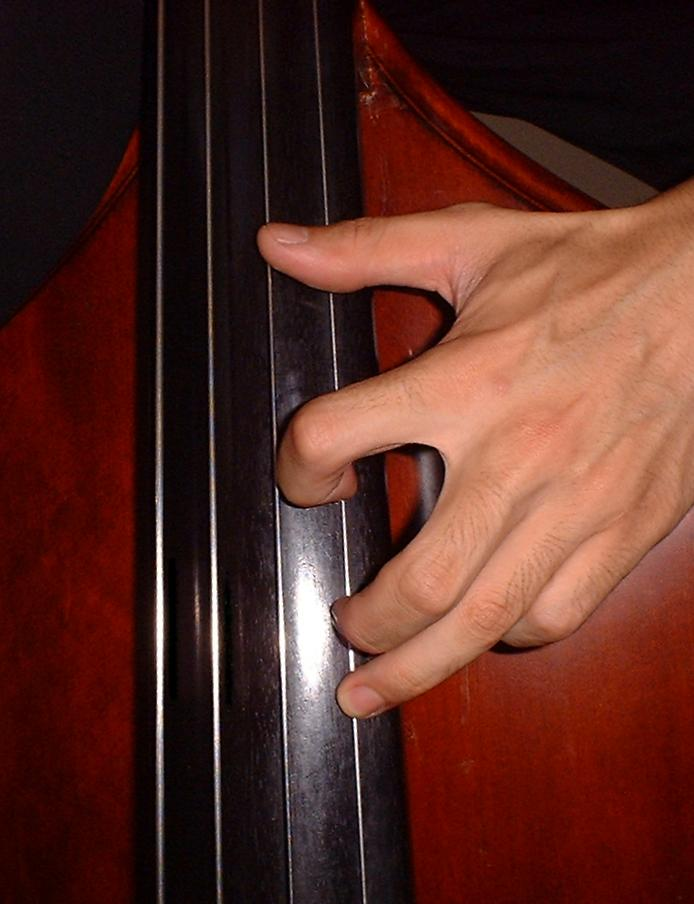
\includegraphics[width=4.5cm]{../Vol1/Pics/Thumb/4th.epsi}\\
{\small 図\thefigure : 全音-全音-半音\\}
\end{center}
\end{minipage}
\end{flushleft}

\subsection{音階練習}

\begin{music}
\nostartrule
\parindent 0pt
\setclef1{\bass}
\generalsignature{0}    
\startpiece
\notes\zchar{14}{ハ長調(C-dur)音階}\enotes
\Notes\zchar{10}{\bf 2}\qu{'C}\enotes
\notes\ibu{0}{'D}{3}\islurd{0}{D}\qb{0}{D}\tbu{0}\tslur{0}{E}\qb{0}{E}\enotes
\notes\ibl{0}{'F}{3}\qb{0}{F}\qb{0}{G}\qb{0}{!a}\tbl{0}\qb{0}{b}\enotes
\bar
\Notes\zchar{12}{\bf 1}\ql{c}\enotes
\notes\ibl{0}{d}{3}\isluru{0}{d}\qb{0}{d}\tbl{0}\tslur{0}{e}\zchar{14}{\bf 2}\qb{0}{e}\enotes
\notes\ibl{0}{f}{3}\qb{0}{f}\flag{16}{17}\qb{0}{g}\zchar{17}{\bf 1}\qb{0}{'a}\tbl{0}\zchar{18}{\bf 2}\qb{0}{b}\enotes
\bar
\Notes\zchar{19}{\bf 3}\ql{'c}\enotes
\notes\ibl{0}{'b}{-2}\isluru{0}{b}\zchar{18}{\bf 2}\qb{0}{b}\tbl{0}\tslur{0}{a}\zchar{17}{\bf 1}\qb{0}{a}\enotes
\notes\ibl{0}{g}{-3}\flag{16}{17}\qb{0}{g}\zchar{15}{\bf 4}\qb{0}{f}\qb{0}{e}\tbl{0}\zchar{13}{\bf 4}\qb{0}{d}\enotes
\bar
\notes\ibl{0}{c}{-3}\qb{0}{c}\zchar{11}{\bf 4}\qb{0}{b}\qb{0}{a}\tbl{0}\qb{0}{'G}\enotes
\notes\ibu{0}{'F}{-3}\qb{0}{F}\qb{0}{E}\qb{0}{D}\tbu{0}\qb{0}{C}\enotes
\endpiece
\end{music}

\subsection{親指基本ポジションのクローズ形、完全四度形で弾ける名曲}
\subsubsection*{ヴェルディ: 歌劇「リゴレット」第1幕第2場より\footnote{道化師リゴレットに殺し屋スパラフチーレが自己紹介する場面。}}
\begin{music}
\nostartrule
\setclef1{\bass}
\generalsignature{-1}    
\generalmeter{\meterC}
\parindent 0pt
\startpiece\bigaccid
\notes\zchar{22}{\bf Andante mosso (\metron{\qu}{66})}\zchar{18}{\it con sord.}\zchar{-3}{\ppp}\enotes
\notes\ibl{0}{b}{0}\isluru{0}{c}\zchar{13}{\downbow}\qb{0}{c}\zchar{-2}{\icresc}\qb{0}{=bc}\tbl{0}\qb{0}{b}\enotes
\notes\ibl{0}{c}{0}\zchar{15}{\upbow}\qb{0}{c^cd}\tbl{0}\tslur{0}{e}\zchar{-2}{\tcresc}\qb{0}{e}\enotes
\bar
\Notes\isluru{0}{f}\zchar{16}{\downbow}\qlp{f}\enotes
\notes\cl{e}\enotes
\Notes\zchar{17}{\upbow}\qlp{g}\enotes
\notes\tslur{0}{f}\cl{f}\enotes
\bar
\Notes\isluru{0}{c}\zchar{14}{\downbow}\qlp{c}\enotes
\notes\cl{=b}\enotes
\Notes\zchar{14}{\upbow}\qlp{d}\enotes
\notes\tslur{0}{c}\cl{c}\enotes
\bar
\Notes\isluru{0}{b}\zchar{12}{\downbow}\qlp{_b}\enotes
\notes\cl{'G}\enotes
\Notes\zchar{12}{\upbow}\qlp{!_a}\enotes
\notes\tslur{0}{'F}\cl{F}\enotes
\alaligne
\Notes\isluru{0}{'G}\zchar{11}{\downbow}\qlp{G}\enotes
\notes\cl{!=a}\enotes
\Notes\zchar{12}{\upbow}\qlp{b}\enotes
\notes\tslur{0}{c}\cl{c}\enotes
\bar
\Notes\isluru{0}{f}\zchar{16}{\downbow}\qlp{f}\enotes
\notes\cl{e}\enotes
\Notes\zchar{17}{\upbow}\qlp{g}\enotes
\notes\tslur{0}{f}\cl{f}\enotes
\bar
\Notes\isluru{0}{c}\zchar{15}{\downbow}\qlp{c}\enotes
\notes\cl{=b}\enotes
\Notes\zchar{16}{\upbow}\qlp{d}\enotes
\notes\tslur{0}{c}\cl{c}\enotes
\bar
\Notes\isluru{0}{b}\zchar{15}{\downbow}\qlp{_b}\enotes
\notes\cl{a}\enotes
\Notes\zchar{12}{\upbow}\qlp{b}\enotes
\notes\cl{'G}\enotes
\alaligne
\Notes\tslur{0}{'F}\zchar{10}{\downbow}\qlp{F}\enotes
\notes\isluru{0}{e}\zchar{-3}{\icresc}\zchar{15}{\upbow}\cl{e}\enotes
\Notes\qlp{f}\enotes
\notes\tslur{0}{e}\cl{e}\enotes
\bar
\Notes\isluru{0}{f}\zchar{16}{\downbow}\qlp{f}\enotes
\notes\cl{e}\enotes
\Notes\zchar{16}{\upbow}\qlp{f}\enotes
\notes\tslur{0}{e}\cl{e}\enotes
\bar
\Notes\isluru{0}{f}\zchar{16}{\downbow}\qlp{f}\zchar{-3}{\tcresc \it cresc.}\enotes
\notes\cl{e}\enotes
\Notes\zchar{16}{\upbow}\qlp{f}\enotes
\notes\tslur{0}{f}\cl{f}\enotes
\bar
\notes\zchar{-3}{\icresc}\zchar{20}{\downbow}\zchar{18}{\bf 4}\usf{g}\ql{_g}\zchar{21}{\upbow}\flag{18}{19}\usf{g}\ql{=g}\zchar{19}{\bf 1}\usf{'a}\ql{_a}\zchar{19}{\bf 2}\usf{a}\ql{=a}\enotes
\bar
\notes\zchar{20}{\bf 3}\usf{'b}\ql{_b}\zchar{20}{\bf 2}\usf{b}\ql{=b}\isluru{0}{c}\zchar{-3}{\tcresc}\zchar{23}{\downbow}\zchar{21}{\bf 3}\usf{c}\ql{c}\zchar{-3}{\icresc}\zchar{20}{\bf 1}\usf{a}\ql{a}\enotes
\bar
\notes\zchar{16}{\upbow}\ql{f}\tslur{0}{c}\ql{c}\zchar{-3}{\tdecresc}\enotes
\Notes\isluru{0}{d}\zchar{-3}{\pp}\zchar{15}{\downbow}\hl{_d}\enotes
\bar
\Notes\zchar{15}{\upbow}\hl{=d}\zchar{15}{\downbow}\hl{e}\enotes
\bar
\notes\tslur{0}{f}\ql{f}\qp\enotes
\Notes\hp\enotes
\setdoublebar\endpiece
\end{music}
